% Copyright (C) 2007 Technical University of Liberec.  All rights reserved.
%
% Please make a following reference to Flow123d on your project site if you use the program for any purpose,
% especially for academic research:
% Flow123d, Research Centre: Advanced Remedial Technologies, Technical University of Liberec, Czech Republic
%
% This program is free software; you can redistribute it and/or modify it under the terms
% of the GNU General Public License version 3 as published by the Free Software Foundation.
%
% This program is distributed in the hope that it will be useful, but WITHOUT ANY WARRANTY;
% without even the implied warranty of MERCHANTABILITY or FITNESS FOR A PARTICULAR PURPOSE.
% See the GNU General Public License for more details.
%
% You should have received a copy of the GNU General Public License along with this program; if not,
% write to the Free Software Foundation, Inc., 59 Temple Place - Suite 330, Boston, MA 021110-1307, USA.
%
%%%%%%%%%%%%%%%%%%%%%%%%%%%%%%%%%%%%%%%%%%%%%%%%%%%%%%%%%%%%%%%%%%
%
% use PDFLatex to compile this
%

\documentclass[a4paper]{article}
\usepackage{amsfonts,amsmath,amsthm,authblk}
\usepackage[bbgreekl]{mathbbol}
\usepackage{stmaryrd}
\usepackage{tikz}
\usepackage{graphicx} %[dvips]
\usepackage[numbers]{natbib}
\usepackage{ mathrsfs }


%%%%%%%%%%%%%%%%%%%%%%%%%%%%%%%%%%%%%%%%%%%%%%%%%%%%%%%%%%%%%%%%%%%%%%%%%%%%
\newtheorem{theorem}{Theorem}[section]
\newtheorem{corollary}[theorem]{Corollary}
\newtheorem{lemma}[theorem]{Lemma}
\newtheorem*{remark}{Remark}
\numberwithin{equation}{section}

%%%%%%%%%%%%%%%%%%%% authors' specific math macros
\def\adiv{\widetilde\div}
\def\aep{\tilde\ep}
\def\agrad{\widetilde\nabla}
\def\avg#1{\left\{\mskip-5mu\left\{#1\right\}\mskip-5mu\right\}}
\def\bbeta{\boldsymbol{\beta}}
\def\CC{\tn C}
\def\d {\,{\rm d}}
\def\ddt#1{\frac{\d #1}{\d t}}
\def\div{\operatorname{div}}
\def\dt{\prtl_t}
\def\dual#1#2{\left\langle #1,#2\right\rangle}
\def\ee{\vc e}
\def\ep{\boldsymbol\varepsilon}
\def\FF{\vc F}
\def\ff{\vc f}
\def\Hf{\mathscr{L}} % Lebesgue space for flow
\def\jmp#1{\left\llbracket #1 \right\rrbracket}
\def\nn{\vc n}
\def\nnu{\boldsymbol\nu}
\def\norm#1{\left\|#1\right\|}
\def\pbar{\overline p}
\def\pphi{{\varphi}}
\def\prtl{\partial}
\def\qq{\vc q}
\def\Real{{\mathbf R}} % set of all real numbers
\def\tn#1{{\mathbb{#1}}}    % tensor
\def\ttraction{\vc t}
\def\U{\vc U}
\def\ubar{\overline\uu}
\def\uu{\vc u}
\def\V{\vc V}
\def\Vel{{\boldsymbol{\mathcal V}}} % Sobolev space for elasticity
\def\Vf{{\mathcal V}} % Sobolev space for flow
\def\vc#1{\mathbf{#1}}     % vector
\def\vv{\vc v}
\def\weakly{\rightharpoonup}
\def\xx{\vc x}
\def\yy{{\vc y}}

% plus and minus in circle
\newcommand{\opm}{
  {\mathbin{
    \mathchoice
      {\buildcirclepm{\displaystyle     }{0.14ex}{0.95}{0.05ex}{.7}}
      {\buildcirclepm{\textstyle        }{0.14ex}{0.95}{0.05ex}{.7}}
      {\buildcirclepm{\scriptstyle      }{0.13ex}{0.955}{0.04ex}{.55}}
      {\buildcirclepm{\scriptscriptstyle}{0.08ex}{0.95}{0.03ex}{.45}}
  }} 
}
\newcommand\buildcirclepm[5]{%
  \begin{tikzpicture}[baseline=(X.base), inner sep=-#5, outer sep=-.65]
    \node[draw,circle,line width=#4] (X)  {\footnotesize\raisebox{#2}{\scalebox{#3}{$#1\pm$}}};
  \end{tikzpicture}%
}

% abbreviations of equation environments
\newcommand{\eq}[1]{\begin{equation}#1\end{equation}}
\newcommand{\eqs}[1]{\begin{equation*}#1\end{equation*}}
\newcommand{\ml}[1]{\begin{multline}#1\end{multline}}
\newcommand{\mls}[1]{\begin{multline*}#1\end{multline*}}

%%%%%%%%%%%%%%%%%%%% end authors' specific math macros


%%%%%%%%%%%%%%%%%%%%%%%%%%%%%%%%%%%%%%%%%%%%%%%%%%%%%%%%%%%%%%%%%%%%%%%%%%%%%%%%%%%%%%%%%%%%% BEGIN DOCUMENT
\begin{document}

\title{Mixed-dimensional models of poroelasticity\thanks{The paper was created with support of project ``RINGEN - research
infrastructure upgrade'' No CZ.02.1.01/0.0/0.0/16\_013/0001792,
co-funded by the EU Operational Programme ``Research, Development and Education''.}}
\author{Jan Březina}
\author{Jan Stebel}
\affil{Institute of New Technologies and Applied Informatics\authorcr
Faculty of Mechatronics, Informatics and Interdisciplinary Studies\authorcr
% Technical University of Liberec
% \authorcr
and\authorcr
Department of Nanotechnology and Informatics\authorcr
Institute for Nanomaterials, Advanced Technologies and Innovation\authorcr
Technical University of Liberec\authorcr
Studentská 1402/2, 461 17 Liberec, Czech Republic\authorcr
\texttt{\{jan.brezina,jan.stebel\}@tul.cz}}
\date{April 3, 2020}
\maketitle

\begin{abstract}
The paper deals with derivation and analysis of a poroelasticity model in a domain with lower-dimensional fracture.
The resulting system of equations, which is obtained by dimension reduction, consists of saturated flow and linear elasticity both in the domain and in the fracture, and of appropriate interface conditions.
Existence and uniqueness of a weak solution is proved with help of a fixed-point argument.
\end{abstract}

\paragraph{Keywords:}
Biot's poroelasticity, dimension reduction, fixed-stress splitting.

\paragraph{2010 Mathematics Subject Classification:}
35M33, % Initial-boundary value problems for mixed-type systems of PDEs
35Q86, % PDEs in connection with geophysics
74S05, % Flows in porous media; filtration; seepage
74F10. % Fluid-solid interactions (including aero- and hydro-elasticity, porosity, etc.)
% 74B05, % Classical linear elasticity
% 74G25, % Existence of solutions of equilibrium problems in solid mechanics


\section{Introduction}

% HIGHLIGHTS:
% \begin{itemize}
% \item Dimension reduction for Biot's poroelasticity based on special tangential and normal calculus.
% \item Dimension reduction for Darcian flow with general anisotropic conductivity tensor.
% \item Existence analysis for mixed-dimensional elasticity using special Korn-type inequality in mixed-dimensional function spaces.
% \item Convergence of fixed-stress iterations and existence of unique solution for ``permeable fracture'' model.
% \end{itemize}


The interaction of fluid flow and rock mechanics plays a significant role in many important applications such as geothermal power utilization, nuclear waste deposition or CO${}_2$ storage \cite{rutqvist2003role}.
Appropriate mathematical models must take into account heterogeneities and fault zones of various scales and shapes.
An important role is played by models describing fractures as codimension-one manifolds, greatly simplifying the treatment of extremely different geometrical scales.
The challenge in mathematical and numerical methods for these problems is very often related to opposite character of flow and mechanics: intact rock (matrix) is stiff but almost impermeable, while fractures are permeable and with small or negligible elastic modulus.
It turns out that simply neglecting the less dominant of these two processess often leads to inaccurate description.
For example, the widely-used \textit{discrete fracture network} (DFN) models are not able to capture the mass transfer between fractures that are not topologically connected.
The communication between fractures and matrix is a part of so-called \textit{discrete fracture-matrix} (DFM) models, also called \textit{mixed-dimensional}.
In modelling hydro-geomechanical coupling, the mechanical response of fractures is often neglected.
However, phenomena like shear-induced opening, friction or healing may play essential role, raising the need for appropriate mathematical description of fracture mechanics.
Our aim is to develop a mixed-dimensional model taking into accout both flow and mechanics in matrix and fractures.

The original idea of dimension reduction comes from \cite{martin_modeling_2005}, where it was applied to Darcian flow and one separating fracture.
Later on the model has been extended e.g. by \cite{angot2009asymptotic} for immersed, polygonal fracture with variable aperture.
DFN models with intersections and junctions were analyzed in e.g. \cite{maryska2005numerical,pichot2012generalized,formaggia2014reduced}, for results on DFM we refer to \cite{schwenck2015dimensionally}.
% 
Mixed-dimensional poroelasticity models were studied e.g. in \cite{ganis2014modeling} where Biot's system in matrix was coupled with fracture flow based on the cubic law.
In \cite{hanowski2018hydromechanical} the Biot system in matrix is coupled with Darcian flow, but in addition fracture width and length can vary according to rock deformation.
Concerning mechanics in fracture, there are not so many papers on dimension reduction.
A general framework for mixed-dimensional elliptic equations was developed in \cite{boon2017functional,boon2019stable} and applied to linear elasticity systems.
We also mention the work \cite{mikelic2019derivation} where a shell model is derived for poroelastic membrane.

In this paper we describe a dimension reduction process for the Biot system in a domain separated by a fracture.
To cope with the fact that the mechanical part of the problem is a system of equations, we develop a special calculus for tangential and normal parts of functions and operators.
In contrast to other works, we also consider general conductivity and elasticity tensors not necessarily aligned with the fracture orientation.
The obtained equations are expressed in terms of mean pressure and mean displacement in the fracture.
The resulting problem consists of equations of flow and mechanics in the fracture and in the surrounding domain, accompanied by appropriate interface conditions.

The second part of the paper deals with the analysis of well-posedness of the mixed-dimensional poroelasticity.
There are two main strategies of solving poromechanics systems: monolithic methods (see e.g. \cite{showalter2000diffusion,zenisek1984existence}) and iterative splittings.
The latter approach has a great advantage in the design of numerical methods where the splitting acts as a preconditioner \cite{white2016block} that allows sequential use of different solvers for flow and mechanics.
Here we follow the optimized fixed-stress iterative splitting proposed in \cite{mikelic2013convergence} and show the contractivity of the appropriate mapping with optimal estimates of splitting parameters.

The structure of the paper is as follows.
In section \ref{sec:model} we describe the full and reduced geometry and the Biot's poroelasticity model.
Then in section \ref{sec:calculus} we present the tangential and normal calculus which will be used in the dimension reduction process in section \ref{sec:dim_red}.
The result of dimension reduction is the system \eqref{eq:mixed_dim_problem}, which describes flow and mechanics in matrix and fracture with appropriate interface conditions.
We further formulate a modified problem \eqref{eq:mixed_dim_perm}, which is valid under the assumption of permeable fracture.
In section \ref{sec:well_pos} we analyze the existence and uniqueness of solution to the latter problem, first studying separately the mechanics and flow and later on combining them in the iterative scheme.


\section{Biot's poroelasticity in domain with fracture}\label{sec:model}

Let $\Omega$ be a bounded, simply connected domain in the Euclidean space $\Real^d$, $d\in\{2,3\}$, with Lipschitz boundary $\partial\Omega$.
We assume that $\Omega$ is composed of two subdomains: the fracture $\Omega_f$ and the matrix $\Omega_m:=\Omega\setminus\overline\Omega_f$, and that the fracture divides the matrix into two parts (see Figure \ref{fig:omegas}).
\begin{figure}[h]
\centering
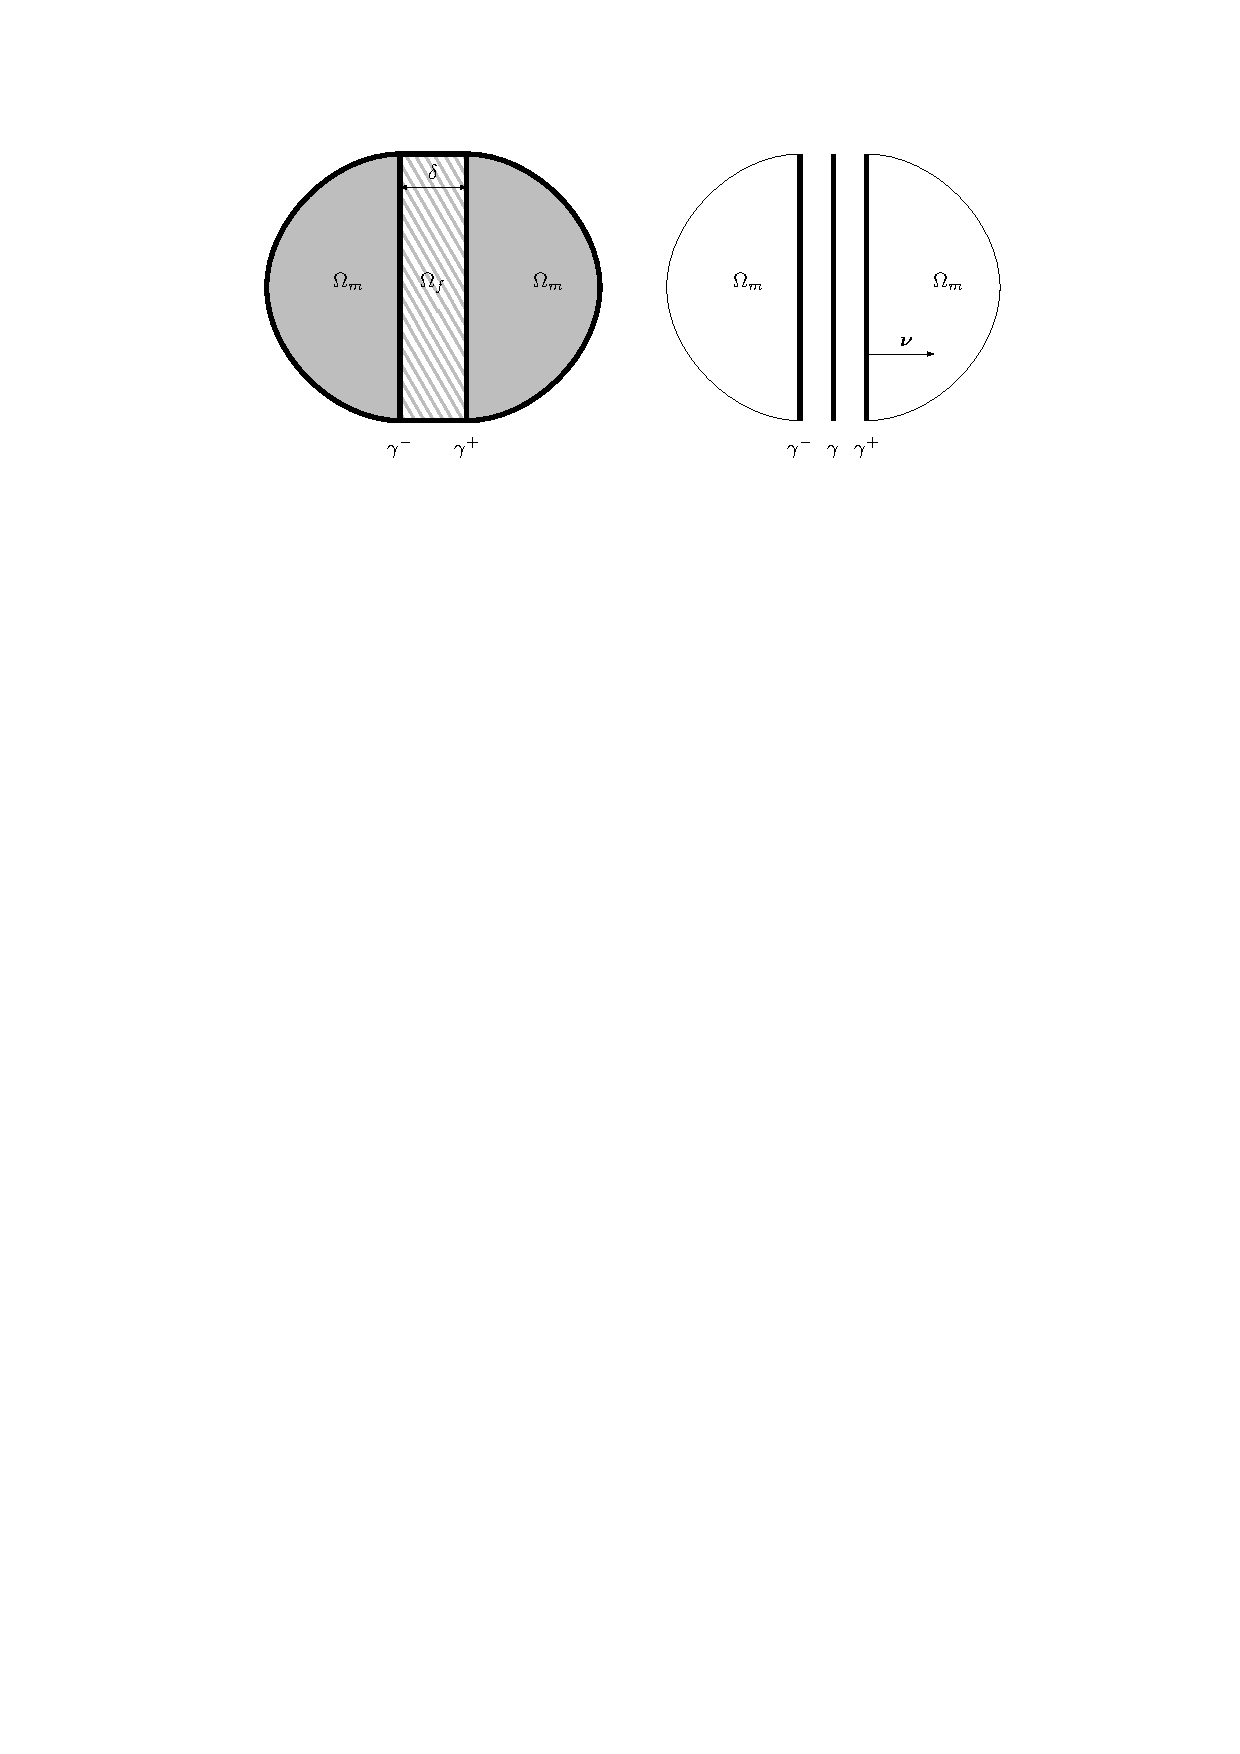
\includegraphics[width=\textwidth]{figures/omegas}
\caption{The domain of the full model (left) and the reduced geometry (right).}
\label{fig:omegas}
\end{figure}
For simplicity we consider a straight fracture, i.e. there is a subset $\gamma$ of a hyperplane in $\Real^d$ with unit normal vector $\nnu$ and a number $\delta>0$ such that
\eqs{ \Omega_f = \{\xx+s\nnu;~\xx\in\gamma,~s\in(-\tfrac\delta2,\tfrac\delta2)\}. }
The parameter $\delta$ is usually called the aperture or the width of the fracture.
Then the two parts of $\Omega_m$ are interacting with $\Omega_f$ via the interfaces
\eqs{ \gamma^+ := \{\xx+\tfrac\delta2\nnu;~\xx\in\gamma\},\quad \gamma^- := \{\xx-\tfrac\delta2\nnu;~\xx\in\gamma\}. }
The symbol $\prtl\gamma$ shall denote the relative boundary of $\gamma$.

The basic hydro-mechanical interaction in a porous medium is described by the Biot system \cite{biot1941general}.
Let $I=(0,T)$ be a finite time interval, $\ff$ the body force, $g$ the fluid source and $p_0$ the initial pressure distribution.
Then the balance of mass and forces in matrix and fracture is given by the equations
\begin{subequations}
\label{eq:biot}
\begin{align}
    \label{eq:lin_el}
    -\div \bbsigma + \nabla(\alpha p) &= \ff &&\mbox{ in }I\times(\Omega_m\cup\Omega_f),\\
\label{eq:biot_darcy}    \dt\left(Sp + \div(\alpha\uu)\right) + \div\qq &= g &&\mbox{ in }I\times(\Omega_m\cup\Omega_f).
\end{align}
Here, the displacement $\uu$ and the pressure $p$ are the principal unknowns; further $\alpha$ is the Biot effective stress parameter, $S$ the storativity.
The stress tensor $\bbsigma$ and the flux $\qq$ are determined by the Hooke and Darcy law, respectively:
\eqs{ \bbsigma = \CC\nabla\uu, \quad \qq = -\tn K\nabla p, }
via the $4^{\rm th}$-order elasticity tensor $\CC$ and the hydraulic conductivity tensor $\tn K$.
We consider the following initial and boundary conditions:
\begin{align}
p(0,\cdot) &= p_0 &&\mbox{ in }\Omega_m\cup\Omega_f,\\
p &= 0,\quad \uu=\vc 0 &&\mbox{ on }I\times\prtl\Omega.
\end{align}
To complete the system of equations, we impose the continuity of pressure, displacement, flux and normal poroelastic stress on the interfaces between matrix and fracture:
\eq{ \label{eq:continuity_on_gamma_pm} p,\uu,\qq\cdot\nnu,\bbsigma\nnu-\alpha p\nnu \mbox{ are continuous on } I\times\gamma^\pm. }
\end{subequations}

In what follows, we shall assume that the physical parameters $\alpha,S,\CC,\tn K$ are constant in $\Omega_m$, $\Omega_f$, respectively.
To distinguish values in $\Omega_m$ and $\Omega_f$, we shall use the subscripts ``$m$'' and ``$f$'', i.e. $\alpha_m := \alpha_{|\Omega_m}$, $\alpha_f := \alpha_{|\Omega_f}$ etc.
We also impose standard requirements for the data:
\begin{itemize}
\item $\alpha_*\ge 0$, $S_*>0$ for $*\in\{m,f\}$;
\item $\CC_*$ and $\tn K_*$, $*\in\{m,f\}$, have the usual symmetries:
\eqs{ \forall \tn A,\tn B\in\Real^{d\times d}:~ \CC_*\tn A:\tn B=\CC_*\tn A^\top:\tn B=\CC_*\tn A:\tn B^\top=\CC_*\tn B:\tn A, }
\eqs{ \tn K_* = \tn K_*^\top; }
\item $\CC_*$ and $\tn K_*$, $*\in\{m,f\}$, are positive definite: % \cite{gurtin}:
There exist positive constants $\mu_m$, $\mu_f$, $\lambda_m$, $\lambda_f$, $\kappa_m$, $\kappa_f$, such that
\eq{ \label{eq:pos_def_C_gen} \forall\tn A\in\Real^{d\times d}:~\CC_*\tn A:\tn A \ge \mu_*\left|\tn A+\tn A^\top\right|^2 + \lambda_*|\tn I:\tn A|^2, }
\eq{ \label{eq:pos_def_K} \forall\vv\in\Real^d:~\tn K_*\vv\cdot\vv \ge \kappa_*|\vv|^2,\quad *\in\{m,f\}. }
\end{itemize}
Here ``:'' stands for the scalar product in $\Real^{d\times d}$ and $|\tn A|$ denotes the Frobenius norm, i.e. $|\tn A|^2=\tn A:\tn A$.




\section{Tangential and normal calculus in fracture}\label{sec:calculus}

In this section we develop tools that will be used later in the derivation of the mixed-dimensional Biot system.
Let $\tn P := \nnu\otimes\nnu = [\nu_i\nu_j]_{i,j=1}^d$ be the orthogonal projector to $\gamma$.
For any $\vv\in\Real^d$ and $\tn A\in\Real^{d\times d}$ we introduce the orthogonal decomposition into normal and tangential direction to $\gamma$:
\eqs{ \vv = \tn P\vv + (\tn I-\tn P)\vv =:\vv_\nu + \vv_\tau, }
\eqs{ \tn A = \tn A\tn P + \tn A(\tn I-\tn P) =: \tn A_\nu + \tn A_\tau. }
In the rest of this section, $f$, $\vv$, $\tn A$ will be scalar-, vector- and tensor-valued functions defined in $\overline\Omega_f$.
The gradient and divergence operators are decomposed into the normal and tangential part as follows:
\eqs{ \nabla f = (\nabla f)_\nu + (\nabla f)_\tau =: \nabla_\nu f + \nabla_\tau f, }
\eqs{ \nabla\vv = (\nabla\vv)_\nu + (\nabla\vv)_\tau =: \nabla_\nu\vv + \nabla_\tau\vv, }
\eqs{ \div\vv = \div\vv_\nu + \div\vv_\tau =: \div_\nu\vv + \div_\tau\vv, }
\eqs{ \div\tn A = \div(\tn P\tn A) + \div((\tn I-\tn P)\tn A) =: \div_\nu\tn A + \div_\tau\tn A. }
We recall that the components of the Jacobian matrix and of the tensor divergence are given by $\nabla\vv=\left[\tfrac{\prtl v_i}{\prtl x_j}\right]_{i,j=1}^d$ and $\div\tn A = \left[\sum_{j=1}^d\tfrac{\prtl a_{ij}}{\prtl x_j}\right]_{i=1}^d$, respectively.
The symbols $f^\oplus$ and $f^\ominus$ will denote the trace of $f$ on $\gamma^+$, $\gamma^-$, respectively, i.e.
\eqs{ f^{\opm}(\xx) := f(\xx\pm\tfrac\delta2\nnu), ~\xx\in\gamma. }
Using these symbols we can introduce the average and jump operators:
\eqs{ \avg{f} := \frac{f^\oplus+f^\ominus}2,\quad \jmp{f} := f^\oplus-f^\ominus. }
The same notation will be used for vector- and tensor-valued functions.
By $\overline f$ we shall denote the integral mean of $f$ across the fracture aperture, i.e.
\eqs{ \overline f(\xx):=\frac1\delta\int_{-\tfrac\delta2}^{\tfrac\delta2} f(\xx+s\nnu) \d s,~\xx\in\gamma. }
The approximate gradient and divergence operators in the positive and negative half of fracture are defined as follows:
\eqs{ \agrad^\opm[f,\overline f] := \nabla_\tau\overline f \pm \frac2\delta(f^\opm - \overline f)\nnu, }
\eqs{ \agrad^\opm[\vv,\overline\vv] := \nabla_\tau\overline\vv \pm \frac2\delta(\vv^\opm - \overline\vv)\otimes\nnu, }
\eqs{ \adiv^\opm[\vv,\overline\vv] := \div_\tau\overline\vv \pm \frac2\delta(\vv^\opm - \overline\vv)\cdot\nnu, }
\eqs{ \adiv^\opm[\tn A,\overline{\tn A}] := \div_\tau\overline{\tn A} \pm \frac2\delta(\tn A^\opm - \overline{\tn A})^\top\nnu. }
\begin{remark}
In the previous definitions we have used two-point differences to approximate derivatives in the normal direction.
We note that it is possible to use more general relations using all three values $f^\oplus$, $\overline f$, $f^\ominus$ (see e.g. \cite{martin_modeling_2005}).
The two-point formulas are suitable for possible generalization at fracture intersections and junctions.
\end{remark}
If $f\in\mathcal C^2(\overline\Omega_f)$, i.e. $f$ is twice continuously differentiable in $\overline\Omega_f$ then from Taylor's expansion we infer that
\eq{ \label{eq:approx_Odelta} f^\opm = \overline f + O(\delta), \quad \nabla f^\opm = \agrad[f,\overline f] + O(\delta), \quad \div f^\opm = \adiv[f,\overline f] + O(\delta). }
Here the remainder $O(\delta)$ represents an expression that can be estimated from above by $\delta C\norm{f}_{\mathcal C^2(\overline\Omega_f)}$ and $C>0$ is a constant independent of $f$ and $\delta$.
Analogous properties hold for vector- and tensor-valued functions.
Despite the indicated approximations, the following relations between the integral means and averaged approximates still hold exactly:
\begin{lemma}
For all admissible functions $f$, $\vv$ and $\tn A$ it holds:
\eq{\label{eq:agrad_sc} \overline{\nabla f} = \nabla_\tau\overline f + \frac1\delta\jmp{f}\nnu = \avg{\agrad[f,\overline f]}, }
\eq{\label{eq:agrad_vc} \overline{\nabla\vv} = \nabla_\tau\overline\vv+\frac1\delta\jmp{\vv}\otimes\nnu = \avg{\agrad[\vv,\overline\vv]}, }
\eq{\label{eq:adiv_vc} \overline{\div\vv} = \div_\tau\overline\vv+\frac1\delta\jmp{\vv}\cdot\nnu = \avg{\adiv[\vv,\overline\vv]}, }
\eq{\label{eq:adiv_tn} \quad \overline{\div\tn A} = \div_\tau\overline{\tn A} + \frac1\delta\jmp{\tn A^\top}\nnu = \avg{\adiv[\tn A,\overline{\tn A}]}. }
\end{lemma}
\begin{proof}
It is readily seen that $\avg{\agrad{f,\overline f}}=\nabla_\tau\overline f + \frac1\delta\jmp{f}$.
Further we have:
\eqs{ \overline{\nabla_\tau f} = \frac1\delta\int_{-\tfrac\delta2}^{\tfrac\delta2}\nabla_\tau f(\cdot+s\nnu) \d s = \nabla_\tau\left(\frac1\delta\int_{-\tfrac\delta2}^{\tfrac\delta2}f(\cdot+s\nnu) \d s\right) = \nabla_\tau\overline f,
}
\eqs{ \overline{\nabla_\nu f} = \frac1\delta\int_{-\tfrac\delta2}^{\tfrac\delta2}\nnu\frac{\rm d}{{\rm d}s}\left(f(\cdot+s\nnu)\right)\d s = \frac1\delta\jmp{f}\nnu,
}
so that $\overline{\nabla f} = \overline{\nabla_\tau f} + \overline{\nabla_\nu f}$ satisfies \eqref{eq:agrad_sc}.
The identities \eqref{eq:agrad_vc}--\eqref{eq:adiv_tn} can be proved analogously.
\end{proof}

We also have the Green identity in $\gamma$:
\eqs{ \int_\gamma(\div_\tau\vv)f = \int_{\prtl\gamma}(\vv\cdot\nn)f - \int_\gamma\vv\cdot\nabla_\tau f, }
where $\nn$ denotes the unit outward normal to $\partial\gamma$.



\section{Dimension reduction}\label{sec:dim_red}

Let us assume that $(\uu,p)$ is a smooth solution of \eqref{eq:biot}.
We shall use the calculus from section \ref{sec:calculus} to derive appropriate equations that are satisfied by the averages $(\ubar,\pbar)$ in $I\times\gamma$.


\subsection{Fracture model for elasticity}\label{sec:reduction_elasticity}

Integrating \eqref{eq:lin_el} over the fracture aperture yields:
\eqs{ -\delta\overline{\div\bbsigma} + \delta\alpha_f\overline{\nabla p} = \delta\overline\ff \mbox{ in }I\times\gamma. }
To express the averaged terms on the left hand side we use \eqref{eq:adiv_tn}, \eqref{eq:agrad_vc} and \eqref{eq:agrad_sc}.
In particular, we obtain:
\eqs{ \overline{\div\bbsigma} = \div_\tau\left(\CC_f\avg{\agrad[\uu,\ubar]}\right) + \frac1\delta\jmp{\CC_f\nabla\uu_{|\Omega_f}}\nnu. }
The normal stress $(\CC_f\nabla\uu_{|\Omega_f})^\opm\nnu$ will be approximated by the quantity
\eq{ \label{eq:def_t} \ttraction^\opm[\uu,\ubar] := \left(\CC_f\agrad^\opm[\uu,\ubar]\right)\nnu. }
Then, taking into account \eqref{eq:approx_Odelta}, we obtain the reduced counterpart of \eqref{eq:lin_el}:
\ml{ \label{eq:lin_el_frac} -\delta\div_\tau\left(\CC_f\avg{\agrad[\uu,\ubar]}\right) + \delta\alpha_f\avg{\agrad[p,\pbar]} - \jmp{\ttraction[\uu,\ubar]}\\
= \delta\overline\ff + O(\delta) \mbox{ in }I\times\gamma. }
The continuity of normal poroelastic stress $\bbsigma\nnu-\alpha p\nnu$ on $\gamma^\pm$ becomes
\eq{ \label{eq:interface_el} (\CC_m(\nabla\uu_{|\Omega_m})^\opm - \alpha_m p^\opm\tn I)\nnu = \ttraction^\opm[\uu,\ubar] - \alpha_f p^\opm\nnu + O(\delta) \mbox{ in }I\times\gamma. }




\subsection{Fracture model for flow}\label{sec:reduction_flow}

Let us integrate \eqref{eq:biot_darcy} over the fracture aperture.
We get:
\eq{ \label{eq:darcy_int} \prtl_t\left(\delta S_f\pbar + \delta\alpha_f\overline{\div\uu}\right) + \delta\overline{\div\qq} = \delta\overline g \mbox{ in }I\times\gamma. }
From \eqref{eq:adiv_vc}, \eqref{eq:agrad_sc} and the definition of $\qq$ we obtain:
\eqs{ \overline{\div\qq} = \div_\tau\overline{\qq} + \frac1\delta\jmp{\qq}\cdot\nnu
= -\div_\tau\left(\tn K_f\avg{\agrad[p,\pbar]}\right) + \frac1\delta\jmp\qq\cdot\nnu. }
To express the approximation of the normal flux $-\qq^\opm\cdot\nnu$ we use the quantity
\eq{ \label{eq:def_F} \pphi^\opm[p,\pbar] := \tn K_f\agrad^\opm[p,\pbar]\cdot\nnu. }
Hence, we obtain from \eqref{eq:darcy_int}--\eqref{eq:def_F} and \eqref{eq:adiv_vc} the reduced flow equation:
\ml{ \label{eq:flow_frac} \delta\prtl_t\left(S_f\pbar + \alpha_f\avg{\adiv[\uu,\ubar]}\right) -\delta\div_\tau\left(\tn K_f\avg{\agrad[p,\pbar]}\right) - \jmp{\pphi[p,\pbar]}\\
= \delta\overline g + O(\delta) \mbox{ in }I\times\gamma. }
Continuity of flux through $\gamma^\pm$ yields:
\eq{ \label{eq:interface_flow} \tn K_m(\nabla p_{|\Omega_m})^\opm\cdot\nnu = \pphi^\opm[p,\pbar] + O(\delta) \mbox{ in }I\times\gamma. }


\subsection{Mixed-dimensional poroelasticity}

The mixed-dimensional coupled problem is obtained after neglecting the remainders $O(\delta)$ in \eqref{eq:lin_el_frac}, \eqref{eq:interface_el}, \eqref{eq:flow_frac}, \eqref{eq:interface_flow}.
Analysis of the truncation error can be done similarly as in \cite{brezina2015analysis}, however in this paper we omit it.
Let $\Gamma:=\prtl\Omega_m\cap\prtl\Omega$, $P_0:=\overline p_0$, $\FF:=\delta\overline\ff$ and $G:=\delta\overline g$.
We want to find functions $\uu,p$ defined in $I\times\Omega_m$ and $\U,P$ defined in $I\times\gamma$, which satisfy:
\begin{subequations}\label{eq:mixed_dim_problem}
\begin{itemize}
\item[(i)] Biot's equations for the matrix:
\begin{align}
\label{eq:mixed_dim_problem_el_mat} -\div(\CC_m\nabla\uu) + \alpha_m\nabla p &= \ff &&\mbox{ in }I\times\Omega_m,\\
\label{eq:mixed_dim_problem_fl_mat}\dt\left(S_m p + \alpha_m\div\uu\right) - \div(\tn K_m\nabla p) &= g &&\mbox{ in }I\times\Omega_m,
\end{align}

\item[(ii)] averaged Biot's equations for the fracture:
\ml{ \label{eq:mixed_dim_problem_el_frac} -\delta\div_\tau\left(\CC_f\avg{\agrad[\uu,\U]}\right) + \delta\alpha_f\avg{\agrad[p,P]} - \jmp{\ttraction[\uu,\U]}\\
 = \FF \mbox{ in }I\times\gamma, }
\ml{ \label{eq:mixed_dim_problem_fl_frac} \delta\prtl_t\left(S_f P + \alpha_f\avg{\adiv[\uu,\U]}\right) -\delta\div_\tau\left(\tn K_f\avg{\agrad[p,P]}\right)\\ - \jmp{\pphi[p,P]}
= G \mbox{ in }I\times\gamma, }

\item[(iii)] interface conditions:
\begin{align}
\label{eq:mixed_dim_problem_int_el} (\CC_m(\nabla\uu)^\opm-\alpha_m p^\opm\tn I)\nnu &= \ttraction^\opm[\uu,\U] - \alpha_f p^\opm\nnu && \mbox{ in }I\times\gamma,\\
\label{eq:mixed_dim_problem_int_fl} \tn K_m(\nabla p)^\opm\cdot\nnu &= \pphi^\opm[p,P] && \mbox{ in }I\times\gamma,
\end{align}

\item[(iv)] boundary conditions:
\begin{align}
\label{eq:mixed_dim_problem_bc_mat} \uu &= \vc 0, \quad p = 0 &&\mbox{ on }I\times\Gamma,\\
\label{eq:mixed_dim_problem_bc_frac}\U &= \vc 0, \quad P = 0 &&\mbox{ on }I\times\prtl\gamma,
\end{align}

\item[(v)] initial conditions:
\begin{align}
p(0,\cdot) &= p_0 &&\mbox{ in }\Omega_m,\\
\label{eq:mixed_dim_problem_init_frac} P(0,\cdot) &= P_0 &&\mbox{ in }\gamma.
\end{align}
\end{itemize}
\end{subequations}
We point out that $\U$ and $P$ play the role of approximations of the averages $\ubar$ and $\pbar$ in $\Omega_f$.

At this moment we note that the problem \eqref{eq:mixed_dim_problem} is not suitable for further analysis.
Namely, formal calculations (see appendix \ref{sec:app_energy_eq}) lead to the following ``energy equality'':
\ml{ \label{eq:apriori_biot} \int_{\Omega_m}\CC_m\nabla\dt\uu:\nabla\dt\uu + \delta\int_\gamma\avg{\CC_f\agrad[\dt\uu,\dt\U]:\agrad[\dt\uu,\dt\U]}\\
+ S_m\int_{\Omega_m}|\dt p|^2 + \delta S_f\int_\gamma|\dt P|^2
+ \frac12\ddt{}\int_{\Omega_m}\tn K_m\nabla p\cdot\nabla p\\
+ \frac\delta2\ddt{}\int_\gamma\avg{\tn K_f\agrad[p,P]\cdot\agrad[p,P]}
+ \int_\gamma\alpha_f\jmp{\dt p\dt(\U-\uu) + \dt P\dt\uu}\cdot\nnu\\
= \int_{\Omega_m}(\dt\ff\cdot\dt\uu + \dt g \dt p) + \int_\gamma(\dt\FF\cdot\dt\U + \dt G \dt P). }
If the the last term on the left hand side was not present, the identity would yield a priori bounds of the solution.
However, this last term cannot be estimated by the other terms and may possibly be a source of uncontrolled ``energy''.
Due to this fact we are unable to prove the global in time existence of weak solution without any further restriction of the model data.





\subsection{Permeable fracture}
In what follows we shall consider the case when the fracture is much more permeable compared to the matrix, in particular that the largest eigenvalue of $\tn K_m$ is much smaller than the smallest eigenvalue of $\tn K_f$:
\eqs{ \lambda_{max}(\tn K_m) \ll \lambda_{min}(\tn K_f). }
Under such conditions the variation of pressure across the fracture width is usually very small compared to the tangential direction.
In the mixed-dimensional setting it means that
\eqs{ \frac1\delta|\jmp{p}| \ll |\nabla_\tau P| \mbox{ and } P \approx p^\opm. }
Then, the last term on the left of \eqref{eq:apriori_biot} becomes negligible:
\mls{ \int_\gamma\alpha_f\jmp{\dt p\dt(\U-\uu) + \dt P\dt\uu}\cdot\nnu\\
= \delta\int_\gamma\alpha_f\dt\left(\frac1\delta\jmp{p}\right)\dt\U\cdot\nnu + \int_\gamma\alpha_f\jmp{\dt (P-p) \dt\uu}\cdot\nnu \approx 0. }
Motivated by the above considerations, we replace the elasticity equation \eqref{eq:mixed_dim_problem_el_frac} and the interface condition \eqref{eq:mixed_dim_problem_int_el} by the following equations:
\eq{ \label{eq:mixed_dim_problem_el_frac_perm} \tag{\ref{eq:mixed_dim_problem_el_frac}'} -\delta\div_\tau\left(\CC_f\avg{\agrad[\uu,\U]}\right) + \delta\alpha_f\nabla_\tau P - \jmp{\ttraction[\uu,\U]} = \FF \mbox{ in }I\times\gamma, }
\eq{ \label{eq:mixed_dim_problem_int_el_perm} \tag{\ref{eq:mixed_dim_problem_int_el}'} (\CC_m(\nabla\uu)^\opm - \alpha_m p^\opm\tn I)\nnu = \ttraction^\opm[\uu,\U] - \alpha_f P\nnu\mbox{ in }I\times\gamma. }
The mixed-dimensional Biot system for permeable fracture, which will be analyzed in the next section, reads as follows:
\eq{ \label{eq:mixed_dim_perm} %\tag{P}
\begin{minipage}{0.85\textwidth}
Find a quadruplet $(\uu,\U,p,P)$ which satisfies \eqref{eq:mixed_dim_problem_el_mat}--\eqref{eq:mixed_dim_problem_fl_mat}, \eqref{eq:mixed_dim_problem_el_frac_perm}, \eqref{eq:mixed_dim_problem_fl_frac}, \eqref{eq:mixed_dim_problem_int_el_perm}, \eqref{eq:mixed_dim_problem_int_fl}--\eqref{eq:mixed_dim_problem_init_frac}.
\end{minipage} }




\section{Well-posedness of mixed-dimensional poroelasticity}\label{sec:well_pos}

In this section we first introduce the weak formulation of \eqref{eq:mixed_dim_perm}.
Then we solve independently the mechanical and the flow part of the problem.
Finally we combine both subproblems in the fixed-stress iterative process and prove its convergence to the solution of the coupled problem.

In what follows we shall use the symbols $L^2(D;Y)$, $H^1(D;Y)$ for the Lebesgue and the Sobolev space of functions defined in $D$ and taking values in $Y$.
If $Y=\Real$ then we shall write simply $L^2(D)$, $H^1(D)$.
Further, $H^1_0(D;Y)$ and $H^1_B(D;Y)$ will be the subspaces of $H^1(D;Y)$ for functions vanishing on the boundary and on a part of boundary $B$, respectively.
The symbol $L^2( I;X)$ will denote the Bochner space and $H^1( I;X)$ its subspace of functions with time derivative in $L^2( I;X)$.
By $\dual{y}{x}_X$ we shall denote the duality pairing between a Banach space $X$ and its dual $X^*$, with $x\in X$ and $y\in X^*$.

For the weak formulation we introduce the spaces
\eqs{ \Vel :=H^1_\Gamma(\Omega_m;\Real^d)\times H^1_0(\gamma;\Real^d), \quad
 \Hf := L^2(\Omega_m)\times L^2(\gamma),\quad \Vf := H^1_\Gamma(\Omega_m)\times H^1_0(\gamma), }
equipped by the norms
\begin{align*}
\norm{(\vv,\V)}_\Vel &:= (\norm{\nabla\vv}_{L^2(\Omega)}^2 + \norm{\nabla_\tau\V}_{L^2(\gamma)}^2)^{1/2},\\
\norm{(q,Q)}_\Hf &:= (\norm{q}_{L^2(\gamma)}^2 + \norm{Q}_{L^2(\gamma)}^2)^{1/2},\\
\norm{(q,Q)}_\Vf &:= (\norm{\nabla q}_{L^2(\gamma)}^2 + \norm{\nabla_\tau Q}_{L^2(\gamma)}^2)^{1/2}.
\end{align*}
Then the weak formulation of \eqref{eq:mixed_dim_perm} reads (see appendix \ref{sec:app_weak_form} for the derivation):


\textit{
Find $(\uu,\U)\in H^1( I;\Vel)$ and $(p,P)\in L^\infty( I;\Vf)\cap H^1( I;\Hf)$ such that
\begin{subequations}
  \label{eq:biot_weak}
  \eq{
    \label{eq:biot_weak-i}
    (p,P)(0,\cdot)=(p_0,P_0);
  }
  for all $(\vv,\V)\in\Vel$ and a.a. $t\in I$:
  \begin{align}
      \notag
      \int_{\Omega_m}\left(\CC_m\nabla\uu:\nabla\vv - \alpha_m p\div\vv\right)\hspace{3.2cm}\\      
      \notag
      + \delta\int_\gamma\avg{\CC_f\agrad[\uu,\U]:\agrad[\vv,\V] - \alpha_f P \adiv[\vv,\V]}\\
      \label{eq:biot_weak-ii}
      = \dual{(\ff,\FF)}{(\vv,\V)}_\Vel;
  \end{align}
  for all $(q,Q)\in\Vf$ and a.a. $t\in I$:
  \begin{align}
      \notag
      \int_{\Omega_m}\left(q\dt(S_m p+\alpha_m\div\uu) + \tn K_m\nabla p\cdot\nabla q\right) \hspace{1cm}\\
      \notag
      + \delta \int_\gamma Q\dt\left(S_f P + \alpha_f\avg{\adiv[\uu,\U]}\right)\\
      \label{eq:biot_weak-iii}
      + \delta \int_\gamma \avg{\tn K_f\agrad[p,P]\cdot\agrad[q,Q]}
      = \dual{(g,G)}{(q,Q)}_\Hf.
  \end{align}
\end{subequations}
}
% 
We state the main result of the paper.
%
\begin{theorem}\label{th:biot_existence}
Let $(\ff,\FF)\in H^1( I;\Vel^*)$, $(g,G)\in L^2( I;\Hf)$ and $(p_0,P_0)\in\Vf$.
Then \eqref{eq:biot_weak} has a unique solution.
\end{theorem}
% 
The proof will be done in the following subsections.



\subsection{Mixed-dimensional linear elasticity}\label{sec:wellposedness_elasticity}

In this section we consider only the mechanical part of the problem \eqref{eq:biot_weak}.
Assuming that $p$ and $P$ are given pressure fields at some time $t\in I$, we define the following forms in $\Vel$:
\eqs{ a((\uu,\U), (\vv,\V)) := \int_{\Omega_m}\CC_m\nabla\uu:\nabla\vv
 + \delta\int_\gamma\avg{\CC_f\agrad[\uu,\U]:\agrad[\vv,\V]}, }
\eqs{ l((\vv,\V)) := \dual{(\ff,\FF)}{(\vv,\V)}_\Vel + \int_{\Omega_m} \alpha_m p\div\vv
  + \delta\int_\gamma \alpha_f P \avg{\adiv[\vv,\V]}. }
Then we introduce the problem:
\eq{ \label{eq:el_weak} \begin{minipage}{0.7\textwidth}
Find $(\uu,\U)\in \Vel$ such that for all $(\vv,\V)\in \Vel$: $a((\uu,\U),(\vv,\V)) = l((\vv,\V))$.
\end{minipage} }
% 
The existence and uniqueness of the solution to \eqref{eq:el_weak} will be proved using the Lax-Milgram theorem.
To ensure ellipticity of the bilinear form $a$, we first prove a suitable inequality for functions in $\Vel$.

\paragraph{Korn type inequalities.}
Let us recall the classical Korn inequality: %(see e.g. \cite{nitsche1981korn}):
For any bounded domain $D\subset\Real^d$ with Lipschitz boundary and a non-trivial part $B\subset\partial D$ there is a constant $C_K:=C_K(D,B)>0$ such that
\eq{ \label{eq:korn} \forall \vv\in H^1_B(D;\Real^d):~C_K\norm{\nabla\vv}_{L^2(D)} \le \norm{\ep(\vv)}_{L^2(D)}, }
where $\ep(\vv):=\frac12(\nabla\vv+(\nabla\vv)^\top)$.
For any function $\V\in H^1(\gamma;\Real^d)$ we denote its symmetrized tangential gradient by
\eqs{ \ep_\tau(\V) := \frac12(\nabla_\tau\V + (\nabla_\tau\V)^\top). }
Similarly for a pair of functions $(\vv,\V)\in\Vel$ we define its symmetrized approximate gradient by
\eqs{ \aep^\opm[\vv,\V] := \frac12(\agrad^\opm[\vv,\V]+(\agrad^\opm[\vv,\V])^\top). }
We have the following Korn inequality in $H^1_0(\gamma)$.
% 
\begin{lemma}\label{th:korn_tau}
There exists a constant $C_1>0$ such that for all $\V\in H^1_0(\gamma;\Real^d)$ it holds:
\eq{ \label{eq:korn_tau} C_1\norm{\nabla_\tau\V}_{L^2(\gamma)}^2 \le \norm{\ep_\tau(\V)}_{L^2(\gamma)}^2. }
\end{lemma}
% 
\begin{proof}
Let $\V\in H^1_0(\gamma;\Real^d)$.
From the definition of the tangential operator it follows that
\eqs{
\norm{\ep_\tau(\V_\nu)}_{L^2(\gamma)}^2 = \tfrac12\norm{\nabla_\tau\V_\nu}_{L^2(\gamma)}^2,
}
which implies
\eqs{%
\norm{\ep_\tau(\V)}_{L^2(\gamma)}^2 = 
\norm{\ep_\tau(\V_\tau)}_{L^2(\gamma)}^2 + \tfrac12\norm{\nabla_\tau\V_\nu}_{L^2(\gamma)}^2. 
}
Further, by mapping $\V$ isometrically from $\gamma$ to a subset of $\Real^{d-1}$, we can apply \eqref{eq:korn} to the tangential part $\V_\tau$, which implies:
\eqs{ \norm{\ep_\tau(\V_\tau)}_{L^2(\gamma)}^2 \ge C_K\norm{\nabla_\tau\V_\tau}_{L^2(\gamma)}^2. }
Altogether we have:
\eqs{ \norm{\ep_\tau(\V)}_{L^2(\gamma)}^2 \ge \min\{C_K,\tfrac12\}\norm{\nabla_\tau\V}_{L^2(\gamma)}^2, }
which proves \eqref{eq:korn_tau}.
\end{proof}

Now we can prove a variant of the Korn inequality in $\Vel$, which takes into account the approximate gradient.
\begin{lemma}
There exists a constant $C_2>0$ such that for all $(\vv,\V)\in \Vel$ it holds:
\eq{\label{eq:korn_frac} C_2\norm{(\vv,\V)}_\Vel^2 \le \norm{\ep(\vv)}_{L^2(\Omega_m)}^2 + \avg{\norm{\aep[\vv,\V]}_{L^2(\gamma)}^2}. }
\end{lemma}
\begin{proof}
Let us assume for contradiction that there is a sequence $\{(\vv_n,\V_n)\}_{n=1}^\infty$ in $\Vel$ such that
\eq{\label{eq:korn_asm_contra} \norm{\ep(\vv_n)}_{L^2(\Omega_m)}^2 + \avg{\norm{\aep[\vv_n,\V_n]}_{L^2(\gamma)}^2} < \frac1n\norm{(\vv_n,\V_n)}_\Vel^2. }
Without loss of generality we may assume that $\norm{(\vv_n,\V_n)}_\Vel=1$, so that
\eq{\label{eq:korn_weak_vV} (\vv_n,\V_n)\weakly (\vv,\V) \mbox{ weakly in }\Vel, ~n\to\infty, }
where $(\vv,\V)\in \Vel$, passing eventually to a subsequence.
From \eqref{eq:korn_asm_contra} and the Korn inequality in $H^1_\Gamma(\Omega_m;\Real^d)$ it follows that
\eq{\label{eq:korn_strong_v} \vv_n\to\vc 0 \mbox{ strongly in }H^1_\Gamma(\Omega_m;\Real^d),~n\to\infty, }
implying that $\vv=\vc 0$.
From \eqref{eq:korn_asm_contra} it also follows that
\eq{\label{eq:korn_conv_approx_grad} \aep^\opm[\vv_n,\V_n] \to 0 \mbox{ strongly in }L^2(\gamma;\Real^{d\times d}),~n\to\infty. }
Using this together with the definition of $\aep^\opm$, \eqref{eq:korn_weak_vV}, \eqref{eq:korn_strong_v} and the embedding $H^1(\Omega_m)\hookrightarrow L^2(\gamma)$, we obtain:
\eqs{ \ep_\tau(\V) = \pm\frac1\delta(\V\otimes\nnu+\nnu\otimes\V), }
from which it follows that $\V\otimes\nnu+\nnu\otimes\V=\tn 0$ and thus $\V=\vc 0$. 


With help of the compact embedding $H^1(\gamma)\hookrightarrow L^2(\gamma)$ we deduce from \eqref{eq:korn_conv_approx_grad} that $\ep_\tau(\V_n)\to 0$ strongly in $L^2(\gamma;\Real^{d\times d})$, $n\to\infty$.
Lemma \ref{th:korn_tau} then implies that also $\V_n\to\vc 0$ strongly in $H^1_0(\gamma;\Real^d)$, $n\to\infty$.
Finally, having shown the strong convergence of $\{(\vv_n,\V_n)\}_{n=1}^\infty$, we observe that
\eqs{ 1 = \lim_{n\to\infty}\norm{(\vv_n,\V_n)}_\Vel = \norm{(\vv,\V)}_\Vel = 0, }
which is a contradiction.
Therefore the proof is finished.
\end{proof}

\paragraph{Existence and uniqueness of solutions.}
In the following lemma we prove essential properties of $a$ and $l$.
\begin{lemma}\label{th:prop_al}
The bilinear form $a$ is bounded and elliptic in $\Vel$ and the linear form $l$ is bounded in $\Vel$.
In particular, there exist constants $C_3=C_3(C_2,\delta,\mu_m,\mu_f)>0$ and $C_4=C_4(\alpha_m,\alpha_f,\delta,\gamma^+,\gamma^-,\Omega_m)>0$ such that
\eqs{ a((\vv,\V),(\vv,\V)) \ge C_3\norm{(\vv,\V)}_\Vel^2, }
\eqs{ l((\vv,\V)) \le \left(\norm{(\ff,\FF)}_{\Vel^*} + C_4\norm{(p,P)}_\Hf\right)\norm{(\vv,\V)}_\Vel }
for all $(\vv,\V)\in\Vel$.
\end{lemma}
\begin{proof}
The boundedness of $a$ and $l$ is a consequence of the embeddings $H^1(\Omega_m)\hookrightarrow L^2(\gamma^\pm)$ and standard inequalities; we prove only the ellipticity.
For any $(\vv,\V)\in \Vel$ we have:
\eqs{ a((\vv,\V),(\vv,\V)) = \int_{\Omega_m}\CC_m\nabla\vv:\nabla\vv
+ \delta\int_\gamma\avg{\CC_f\agrad[\vv,\V]:\agrad[\vv,\V]}. }
Now we can apply \eqref{eq:pos_def_C_gen} and \eqref{eq:korn_frac}, which yields:
\mls{ a((\vv,\V),(\vv,\V)) \ge 2\mu_m\norm{\ep(\vv)}_{L^2(\Omega_m)}^2 + 2\mu_f\delta\avg{\norm{\aep[\vv,\V]}_{L^2(\gamma)}^2}\\
\ge 2C_2\min\{\mu_m,\mu_f\delta\}\norm{(\vv,\V)}_\Vel^2. }
From this we see that $a$ is elliptic with the constant $C_3 = 2C_2\min\{\mu_m,\mu_f\delta\}$.
\end{proof}
% 
Having shown the above properties of the forms $a$ and $l$, the following result is a direct consequence of the Lax-Milgram theorem.
%
\begin{theorem}
Let $(\ff,\FF)\in\Vel^*$ and $(p,P)\in\Hf$. Then problem \eqref{eq:el_weak} has a unique solution $(\uu,\U)\in\Vel$ which satisfies:
\eqs{
 \norm{(\uu,\U)}_{\Vel} \le \frac{1}{C_3} \Big( \norm{(\ff,\FF)}_{\Vel^*} + C_4\norm{(p,P)}_\Hf \Big).
}
\end{theorem}
% 
Now we consider the time-dependent case.
If $(\ff,\FF,p,P)$ are defined in the time interval $I$, then by differentiating the identity in \eqref{eq:el_weak} with respect to time we observe that the pair $(\dt\uu,\dt\U)$ satisfies for all $(\vv,\V)\in\Vel$:
\eq{ \label{eq:el_dt} a((\dt\uu,\dt\U),(\vv,\V)) = \dt l((\vv,\V)), }
where $\dt l$ stands for the linear form
\mls{ \dt l((\vv,\V)) := \dual{(\dt\ff,\dt\FF)}{(\vv,\V)}_\Vel + \int_{\Omega_m} \alpha_m \dt p\div\vv\\
  + \delta\int_\gamma \alpha_f \dt P \avg{\adiv[\vv,\V]}. }
Similarly as in Lemma \ref{th:prop_al}, one can show that $\dt l$ is bounded and estimate it in terms of the time derivatives of the data:
\eqs{ \dt l((\vv,\V)) \le \left(\norm{(\dt\ff,\dt\FF)}_{\Vel^*} + C_4\norm{(\dt p,\dt P)}_\Hf\right)\norm{(\vv,\V)}_\Vel. }
Since the solution mappings $(\ff,\FF,p,P) \mapsto (\uu, \U)$ and $(\dt\ff,\dt\FF,\dt p,\dt P)\mapsto(\dt\uu,\dt\U)$ are linear and bounded, we obtain:
\begin{corollary}
Let $(\ff,\FF)\in L^2( I;\Vel^*)$ and $(p,P)\in L^2( I;\Hf)$.
Denoting by $(\uu[t],\U[t])$ the solution to \eqref{eq:el_weak} with the data $\ff[t],\FF[t],p[t],P[t]$, then $(\uu,\U)\in L^2( I;\Vel)$.
If in addition $\dt(\ff,\FF)\in L^2( I;\Vel^*)$ and $\dt(p,P)\in L^2( I;\Hf)$, then also $\dt(\uu,\U)\in L^2( I;\Vel)$.
\end{corollary}
% 
Based on the above result, we define the mapping $\mathcal E: H^1( I;\Hf)\to H^1( I;\Vel)$ by the relation
\eqs{ \mathcal E(p,P)[t] := (\uu[t],\U[t]). }
We shall use it in the definition of the fixed-stress splitting in section \ref{sec:iter}.


\subsection{Mixed-dimensional flow}\label{sec:wellposedness_flow}

We now turn to the flow part of the mixed-dimensional problem \eqref{eq:biot_weak}, assuming zero displacements.
We want to solve the following problem:

\textit{Find $(p,P)\in L^\infty( I;\Vf)\cap H^1( I;\Hf)$ such that
\begin{subequations}
    \label{eq:flow_weak}
    \eq{
        \label{eq:flow_weak-i}
        (p,P)(0,\cdot)=(p_0,P_0);
    }
    %    
    and for all $(q,Q)\in\Vf$ and a.a. $t\in I$:
    \begin{align}
      \notag
      \int_{\Omega_m}\left(S_m q\dt p + \tn K_m\nabla p\cdot\nabla q\right) 
      + \delta S_f\int_\gamma Q\dt P \hspace{2cm}\\
      \label{eq:flow_weak-ii}
      + \delta\int_\gamma\avg{\tn K_f\agrad[p,P]\cdot\agrad[q,Q]}
      = \dual{(\tilde g,\tilde G)}{(q,Q)}_\Hf.
    \end{align}
\end{subequations}}
Here $(\tilde g,\tilde G)$ are modified fluid sources to be specified in section \ref{sec:iter}.
The well-posedness of \eqref{eq:flow_weak} will be established on the base of standard theory of parabolic problems (see e.g. \cite{evans_pde}, chap. 7.1).
We formulate the result in the following theorem.
% 
\begin{theorem}
Let $(p_0,P_0)\in\Vf$ and $(\tilde g,\tilde G)\in L^2( I;\Hf)$.
Then there exists a unique solution to \eqref{eq:flow_weak}.
\end{theorem}
\begin{proof}
\underline{Existence:}
Let $\{w_j\}_{j=1}^\infty$ and $\{W_j\}_{j=1}^\infty$ be bases in $H^1_\Gamma(\Omega_m)$, $H^1_0(\gamma)$, respectively, orthonormal with respect to the $L^2$-scalar products.
For any $n=1,2,...$ we define the Galerkin approximation $(p_n,P_n)$ as a pair of functions in the form $p_n(t,\xx):=\sum_{j=1}^n\psi_j^n(t)w_j(\xx)$, $P_n(t,\xx):=\sum_{j=1}^n\Psi_j^n(t)W_j(\xx)$, satisfying for a.a. $t\in I$ and for $i=1,...,n$ the integral identities
\ml{ \label{eq:galerkin_m} S_m\int_{\Omega_m}w_i\dt p_n + \int_{\Omega_m}\tn K_m\nabla p_n\cdot\nabla w_i + \delta\int_\gamma\avg{\tn K_f\agrad[p_n,P_n]\cdot\agrad[w_i,0]}\\
+ \int_\gamma\jmp{\pphi[p_n,P_n]w_i} = \int_{\Omega_m}\tilde g w_i, }
\eq{ \label{eq:galerkin_f} \delta S_f\int_\gamma W_i\dt P_n + \delta\int_\gamma\tn K_f\avg{\agrad[p_n,P_n]}\cdot\nabla_\tau W_i - \int_\gamma\jmp{\pphi[p_n,P_n]W_i} = \int_\gamma \tilde G W_i, }
and the initial conditions
\eqs{ \psi_i(0)=\int_{\Omega_m}p_0w_i, \quad \Psi_i(0)=\int_\gamma P_0W_i. }
The existence and uniqueness of $(p_n,P_n)$ follows from the Carath\'eodory theory of ODEs.
Multiplying \eqref{eq:galerkin_m} by $\psi_i'$ and \eqref{eq:galerkin_f} by $\Psi_i'$, summing over $i=1,...,n$ and integrating in time, we arrive at the identity
\ml{\label{eq:energy_est_1} \norm{\dt(\sqrt{S_m} p_n,\sqrt{\delta S_f} P_n)}_\Hf^2\\
+ \frac12\ddt{}\left(\int_{\Omega_m}\tn K_m\nabla p_n\cdot\nabla p_n
+ \delta\int_\gamma\avg{\tn K_f\agrad[p_n,P_n]\cdot\agrad[p_n,P_n]}\right)\\
= \dual{(\tilde g,\tilde G)}{\dt(p_n,P_n)}_\Vf. }
From the positive definiteness of $\tn K_f$ and the definition of $\agrad^\opm$ we infer that
\eq{ \label{eq:pos_kf_agrad} \avg{\tn K_f\agrad[p_n,P_n]\cdot\agrad[p_n,P_n]} \ge \kappa_f\left(|\nabla_\tau P_n|^2 + \frac2\delta|p_n^\opm-P_n|^2\right). }
Hence, after integrating \eqref{eq:energy_est_1} in time, using the positive definiteness of $\tn K_m$, \eqref{eq:pos_kf_agrad}, the initial conditions and a suitable estimate of the right hand side, we obtain:
\eq{ \label{eq:energy_est_flow} \int_0^T\norm{\dt(p_n,P_n)}_\Hf^2 + \sup_{t\in I}\norm{(p_n,P_n)}_\Vf^2(t) \le C\left(\norm{(p_0,P_0)}_\Vf^2 + \int_0^T\norm{(\tilde g,\tilde G)}_{\Hf}^2\right), }
where $C>0$ may depend on $S_m,S_f,\delta,\kappa_m,\kappa_f,|\tn K_m|,|\tn K_f|$.


Hence the sequence $\{(p_n,P_n)\}_{n=1}^\infty$ is bounded in $L^\infty( I;\Vf)\cap H^1( I;\Hf)$.
Choosing a subsequence weakly convergent in the above spaces to a pair $(p,P)$, we can pass to the limit in \eqref{eq:galerkin_m}--\eqref{eq:galerkin_f}, which proves that $(p,P)$ is a solution of \eqref{eq:flow_weak}.

\underline{Uniqueness:}
Let $(p^1,P^1)$ and $(p^2,P^2)$ be two solutions of \eqref{eq:flow_weak} and denote their difference by $(\Delta p,\Delta P)$.
Subtracting the integral identities in \eqref{eq:flow_weak-ii} for the two solutions and testing by $(\Delta p,\Delta P)$ we obtain:
\ml{ \label{eq:dif_p} \frac12\ddt{}\norm{(\sqrt{S_m}\Delta p,\sqrt{\delta S_f}\Delta P)}_\Hf^2
+ \int_{\Omega_m}\tn K_m\nabla\Delta p\cdot\nabla\Delta p\\
+ \delta\int_\gamma\avg{\tn K_f\agrad[\Delta p,\Delta P]\cdot\agrad[\Delta p,\Delta P]} = 0. }
Since all but the first term on the left hand side of \eqref{eq:dif_p} are nonnegative, we obtain the inequality
\eqs{ \ddt{}\norm{(\Delta p,\Delta P)}_\Hf^2 \le 0, }
which together with the fact that $(\Delta p,\Delta P)(0,\cdot) = (0,0)$ implies $(p^1,P^1)=(p^2,P^2)$.
\end{proof}
% 
Having the above result, we introduce the solution map $\mathcal F:L^2( I;\Hf)\to L^\infty( I;\Vf)\cap H^1( I;\Hf)$ by the relation
\eqs{ \mathcal F(\tilde g,\tilde G) := (p,P), }
where $(p,P)$ is the solution of \eqref{eq:flow_weak}.
Let $\bbeta:=(\beta_m,\beta_f)$ be a pair of positive parameters.
We define a similar map $\mathcal F_{\bbeta}$ as the solution operator for the flow problem with increased storativity $S_m+\beta_m$, $S_f+\beta_f$, respectively.
In particular, $(p,P):=\mathcal F_{\bbeta}(\tilde g,\tilde G)$ satisfies the initial conditions 
\eqref{eq:flow_weak-i} and the integral identity
\ml{ \label{eq:flow_problem_beta} (S_m+\beta_m)\int_{\Omega_m} q\dt p + \int_{\Omega_m}\tn K_m\nabla p\cdot\nabla q + \delta (S_f+\beta_f)\int_\gamma Q\dt P\\
+ \delta\int_\gamma\avg{\tn K_f\agrad[p,P]\cdot\agrad[q,Q]}
= \dual{(\tilde g,\tilde G)}{(q,Q)}_\Hf }
for all $(q,Q)\in\Vf$ and a.a. $t\in I$.



\subsection{Fixed-stress iterations}\label{sec:iter}

We follow the idea of optimized fixed-stress splitting from \cite{mikelic2013convergence}.
Let $\mathcal X := L^\infty( I;\Vf)\cap H^1( I;\Hf)$.
For any $n\in\{0,1,2,...\}$ and $(p^n,P^n)\in \mathcal X$
we define
\eqs{ (\uu^n,\U^n) := \mathcal E(p^n,P^n). }
Next we choose a pair of positive parameters $\bbeta:=(\beta_m,\beta_f)$ and define
\eqs{ (p^{n+1},P^{n+1}) := \mathcal F_{\bbeta}(\tilde g^n,\tilde G^n), }
where
\eqs{ \tilde g^n:=g -\alpha_m\div\dt\uu^n + \beta_m\dt p^n, }
\eqs{ \tilde G^n:=G -\delta\alpha_f\avg{\adiv[\dt\uu^n,\dt\U^n]} + \delta\beta_f\dt P^n. }
From the results of sections \ref{sec:wellposedness_elasticity} and \ref{sec:wellposedness_flow} we infer that whenever $(g,G)\in L^2(I;\Hf)$ then also $(\tilde g^n,\tilde G^n)\in L^2(I;\Hf)$.
The above scheme defines the mapping
\eqs{ \mathcal M_{\bbeta}:(p^n,P^n) \mapsto (p^{n+1},P^{n+1}) }
from $\mathcal X$ into itself.
If $(\hat p,\hat P)$ is a fixed point of this map and $(\hat\uu,\hat\U):=\mathcal E(\hat p,\hat P)$, then $(\hat\uu,\hat\U,\hat p,\hat P)$ is a solution to \eqref{eq:biot_weak}.
Let
\eqs{ \omega:=\min\left\{\frac{S_m+\beta_m}{\beta_m}, \frac{S_f+\beta_f}{\beta_f}\right\}. }
Then the following expression $\rho_{\bbeta}$ is a distance in $\mathcal X$:
\mls{ \rho_{\bbeta}((p_1,P_1),(p_2,P_2))^2 := \frac\omega{\beta_m}\int_0^T\norm{\dt\left(\alpha_m\div(\uu_1-\uu_2)-\beta_m(p_1-p_2)\right)}_{L^2(\Omega_m)}^2\\
+ \frac{\delta\omega}{\beta_f}\int_0^T\avg{\norm{\dt\left(\alpha_f\adiv[\uu_1-\uu_2,\U_1-\U_2]-\beta_f(P_1-P_2)\right)}_{L^2(\gamma)}^2}\\
+ \sup_{t\in I}\left(\kappa_m\norm{\nabla (p_1-p_2)}_{L^2(\Omega_m)}^2 + \delta\kappa_f\avg{\norm{\agrad[p_1-p_2,P_1-P_2]}_{L^2(\gamma)}^2}\right), }
where $(\uu_i,\U_i):=\mathcal E(p_i,P_i)$, $i=1,2$.
Further, $(\mathcal X,\rho_{\bbeta})$ is a complete metric space.
We shall prove that $\mathcal M_{\bbeta}$ is a contraction with respect to $\rho_{\bbeta}$.
Then $\mathcal M_{\bbeta}$ has a unique fixed point and \eqref{eq:biot_weak} has a unique solution, thus Theorem \ref{th:biot_existence} will be proved.
\begin{theorem}\label{th:conv_iter}
Let $(\ff,\FF)\in H^1( I;\Vel^*)$, $(g,G)\in L^2( I;\Hf)$ and $(p_0,P_0)\in\Vf$.
If the pair $\bbeta=(\beta_m,\beta_f)$ satisfies
%
\eq{ 
  \label{eq:cond_beta} 
  \beta_m\ge\frac{\alpha_m^2}{2\left(\frac{2\mu_m}d+\lambda_m\right)}   
  \quad\mbox{and}\quad 
  \beta_f\ge\frac{\alpha_f^2}{2\left(\frac{2\mu_f}d+\lambda_f\right)}, 
}
then $\mathcal M_{\bbeta}$ is a contraction in $\mathcal X$ with respect to the distance $\rho_{\bbeta}$.
Hence the sequence $\{(p^n,P^n)\}_{n=0}^\infty$ with an arbitrary initial guess $(p^0,P^0)\in\mathcal X$, has a unique fixed point $(\hat p,\hat P)$.
Denoting $(\hat \uu,\hat \U):=\mathcal E(\hat p,\hat P)$, then the quadruplet $(\hat \uu,\hat \U,\hat p,\hat P)$ is the unique solution of the coupled problem \eqref{eq:biot_weak}.
The contraction constant takes the value $1/\omega$, which becomes smallest when equalities hold in \eqref{eq:cond_beta}.
\end{theorem}
\begin{proof}
For $n=1,2,...$ we denote:
\begin{align*}
\Delta_p^n&:=p^n-p^{n-1}, \quad e_p^n:=\dt\Delta_p^n,\\
\Delta_P^n&:=P^n-P^{n-1}, \quad e_P^n:=\dt\Delta_P^n,\\
\ee_\uu^n&:=\dt(\uu^n-\uu^{n-1}),\\
\ee_\U^n&:=\dt(\U^n-\U^{n-1}).
\end{align*}
We subtract the equations \eqref{eq:el_dt} for $(\dt\uu^{n+1},\dt\U^{n+1})$ and $(\dt\uu^n,\dt\U^n)$ and test by $(\ee_\uu^{n+1},\ee_\U^{n+1})$.
We obtain:
\mls{ \int_{\Omega_m}\CC_m\nabla\ee_\uu^{n+1}:\nabla\ee_\uu^{n+1}
 + \delta\int_\gamma\avg{\CC_f\agrad[\ee_\uu^{n+1},\ee_\U^{n+1}]:\agrad[\ee_\uu^{n+1},\ee_\U^{n+1}]}\\
 = \int_{\Omega_m} e_p^{n+1} \alpha_m\div\ee_\uu^{n+1} + \delta\int_\gamma e_P^{n+1} \avg{\alpha_f\adiv[\ee_\uu^{n+1},\ee_\U^{n+1}]}. }
Using \eqref{eq:pos_def_C_gen} and the inequalities \eqref{eq:ineq_div_ep}--\eqref{eq:ineq_adiv_aep} from appendix \ref{sec:ap_ineq} we obtain:
\mls{ \left(\frac{2\mu_m}d + \lambda_m\right)\norm{\div\ee_\uu^{n+1}}_{L^2(\Omega_m)}^2 + \delta\left(\frac{2\mu_f}d+\lambda_f\right)\avg{\norm{\adiv[\ee_\uu^{n+1},\ee_\U^{n+1}]}_{L^2(\gamma)}^2}\\
\le \int_{\Omega_m} e_p^{n+1} \alpha_m\div\ee_\uu^{n+1} + \delta\int_\gamma e_P^{n+1} \avg{\alpha_f\adiv[\ee_\uu^{n+1},\ee_\U^{n+1}]}, }
which together with \eqref{eq:cond_beta} yields:
\ml{ 
    \label{eq:ineq_dif_el} 
    \frac1{2\beta_m}\norm{\alpha_m\div\ee_\uu^{n+1}}_{L^2(\Omega_m)}^2 + \frac\delta{2\beta_f}\avg{\norm{\alpha_f\adiv[\ee_\uu^{n+1},\ee_\U^{n+1}]}_{L^2(\gamma)}^2}\\
    %
    - \frac1{\beta_m}\int_{\Omega_m} \beta_m e_p^{n+1}\alpha_m\div\ee_\uu^{n+1} 
    - \frac\delta{\beta_f}\int_\gamma \beta_f e_P^{n+1} \alpha_f\avg{\adiv[\ee_\uu^{n+1},\ee_\U^{n+1}]} \le 0. 
}
Next we subtract the equations \eqref{eq:flow_problem_beta} for $(p^{n+1},P^{n+1})$ and $(p^n,P^n)$ with appropriate right hand sides $(\tilde g^n,\tilde G^n)$ and $(\tilde g^{n-1},\tilde G^{n-1})$, respectively, test by $(e_p^{n+1},e_P^{n+1})$, integrate in time and use \eqref{eq:pos_def_K}, which yields for a.a. $t\in I$:
\ml{ 
    \label{eq:dif_flow_beta} 
    (S_m+\beta_m)\int_0^t\norm{e_p^{n+1}}_{L^2(\Omega_m)}^2 
    + \delta(S_f+\beta_f)\int_0^t\norm{e_P^{n+1}}_{L^2(\gamma)}^2\\
    %
    + \frac{\kappa_m}2\norm{\nabla\Delta_p^{n+1}}_{L^2(\Omega_m)}^2(t) + \frac{\delta\kappa_f}2\avg{\norm{\agrad[\Delta_p^{n+1},\Delta_P^{n+1}]}_{L^2(\gamma)}^2(t)}\\
    %
    \le -\int_0^t\int_{\Omega_m}\underbrace{\left(\alpha_m\div\ee_\uu^n 
    - \beta_m e_p^n\right)}_{=:e_\sigma^n} e_p^{n+1} - \delta\int_0^t\int_\gamma\avg{\underbrace{\alpha_f\adiv[\ee_\uu^n,\ee_\U^n] - \beta_f e_P^n}_{=:e_\Sigma^n}} e_P^{n+1}. 
}
We apply H\"older's and Young's inequality to the right hand side of \eqref{eq:dif_flow_beta} and obtain:
\ml{ 
    \label{eq:dif_flow_beta2}
    \frac{S_m+\beta_m}{\beta_m^2}\int_0^t\norm{\beta_m e_p^{n+1}}_{L^2(\Omega_m)}^2 
    + \delta\frac{S_f+\beta_f}{\beta_f^2}\int_0^t\norm{\beta_f e_P^{n+1}}_{L^2(\gamma)}^2\\
    %
    + \frac{\kappa_m}2\norm{\nabla\Delta_p^{n+1}}_{L^2(\Omega_m)}^2(t) 
    + \frac{\delta\kappa_f}2\avg{\norm{\agrad[\Delta_p^{n+1},\Delta_P^{n+1}]}_{L^2(\gamma)}^2(t)}\\
    %
    \le \frac{S_m+\beta_m}{2\beta_m^2}\int_0^t\norm{\beta_m e_p^{n+1}}_{L^2(\Omega_m)}^2 
    + \frac1{2(S_m+\beta_m)}\int_0^t\norm{e_\sigma^n}_{L^2(\Omega_m)}^2\\
    %
    + \frac{\delta(S_f+\beta_f)}{2\beta_f^2}\int_0^t\norm{\beta_f e_P^n}_{L^2(\gamma)}^2 
    + \frac\delta{2(S_f+\beta_f)}\int_0^t\avg{\norm{e_\Sigma^n}_{L^2(\gamma)}^2}. 
}
%
Subtracting the first and the third term on the right hand side of \eqref{eq:dif_flow_beta2} and estimating the coefficients $(S_*+\beta_*)/\beta_*^2$ from below by $\omega/\beta_*$, $*\in\{m,f\}$, the inequality simplifies as follows:
\ml{
    \label{eq:ineq_dif_flow} 
    \frac\omega{2\beta_m}\int_0^t\norm{\beta_m e_p^{n+1}}_{L^2(\Omega_m)}^2 
    + \frac{\delta\omega}{2\beta_f}\int_0^t\norm{\beta_f e_P^{n+1}}_{L^2(\gamma)}^2\\
    %
    + \frac{\kappa_m}2\norm{\nabla\Delta_p^{n+1}}_{L^2(\Omega_m)}^2(t) 
    + \frac{\delta\kappa_f}2\avg{\norm{\agrad[\Delta_p^{n+1},\Delta_P^{n+1}]}_{L^2(\gamma)}^2(t)}\\
    %
    \le \frac1{2(S_m+\beta_m)}\int_0^t\norm{e_\sigma^n}_{L^2(\Omega_m)}^2
    + \frac\delta{2(S_f+\beta_f)}\int_0^t\avg{\norm{e_\Sigma^n}_{L^2(\gamma)}^2}. 
}
Now we multiply \eqref{eq:ineq_dif_el} by $\omega$, integrate in time and add to \eqref{eq:ineq_dif_flow}.
The square of the difference formula then yields:
\mls{
    \frac\omega{2\beta_m}\int_0^t\norm{e_\sigma^{n+1}}_{L^2(\Omega_m)}^2 
    + \frac{\delta\omega}{2\beta_f}\int_0^t\avg{\norm{e_\Sigma^{n+1}}_{L^2(\gamma)}^2}\\
    %
    + \frac{\kappa_m}2\norm{\nabla\Delta_p^{n+1}}_{L^2(\Omega_m)}^2(t) 
    + \frac{\delta\kappa_f}2\avg{\norm{\agrad[\Delta_p^{n+1},\Delta_P^{n+1}]}_{L^2(\gamma)}^2(t)}\\
    %
    \le \frac1{2(S_m+\beta_m)}\int_0^t\norm{e_\sigma^n}_{L^2(\Omega_m)}^2
    + \frac\delta{2(S_f+\beta_f)}\int_0^t\avg{\norm{e_\Sigma^n}_{L^2(\gamma)}^2}. 
}
%
Using the fact that $\frac1{S_*+\beta_*}\le\frac1{\omega^2}\frac{\omega}{\beta_*}$, $*\in\{m,f\}$, the right hand side of the above inequality can be estimated from above and we obtain:
\mls{ \frac12\left(\rho_{\bbeta}((p^{n+1},P^{n+1}),(p^n,P^n))\right)^2\\
\le \frac1{\omega^2}\left(\frac\omega{2\beta_m}\int_0^t\norm{e_\sigma^n}_{L^2(\Omega_m)}^2
+ \frac{\delta\omega}{2\beta_f}\int_0^t\avg{\norm{e_\Sigma^n}_{L^2(\gamma)}^2}\right)\\
\le \frac1{2\omega^2}\left(\rho_{\bbeta}((p^n,P^n),(p^{n-1},P^{n-1}))\right)^2. }
Hence
\eqs{ \rho_{\bbeta}((p^{n+1},P^{n+1}),(p^n,P^n)) \le \frac1\omega \rho_{\bbeta}((p^n,P^n),(p^{n-1},P^{n-1})). }
It is readily seen that $\omega>1$.
Since $\omega$ is non-increasing with respect to $\beta_m$ and $\beta_f$, the smallest constant of contraction is obtained for the smallest possible values of $\beta_m$, $\beta_f$.
\end{proof}
% 
As we noted above, Theorem \ref{th:conv_iter} implies the existence of a unique solution to \eqref{eq:biot_weak}.
Hence Theorem \ref{th:biot_existence} is proved.



\section*{Conclusion}
We have derived a mixed-dimensional model of flow and linear elasticity in fractured porous media.
Under the assumption of permeable fracture, the existence and uniqueness of weak solution was proved using the fixed-stress splitting scheme.
The convergence of this scheme has been analyzed and optimal values of iteration parameters were found in agreement e.g. with \cite{both2017robust}.
The numerical solution based on the proposed splitting will be the subject of a following paper.
The problem can be further extended to the case of embedded fracture with variable aperture and intersecting fractures, further one should consider contact and friction conditions (such as in \cite{berge2019finite}), to name a few challenging tasks.




\bibliographystyle{abbrvnat}
\bibliography{biot_fracture.bib}



\appendix
% \section{Appendix}

\section{Auxiliary inequalities and identities}\label{sec:ap_ineq}

In what follows we prove some technical relations that are used in the paper.
\begin{lemma}
For all functions $(\vv,\V)\in\Vel$ it holds:
\eq{ \label{eq:ineq_div_ep} \norm{\div\vv}_{L^2(\Omega_m)}^2 \le d\norm{\ep(\vv)}_{L^2(\Omega_m)}^2, }
\eq{ \label{eq:ineq_adiv_aep} \norm{\adiv^\opm[\vv,\V]}_{L^2(\gamma)}^2 \le d\norm{\aep^\opm[\vv,\V]}_{L^2(\gamma)}^2. }
\end{lemma}
\begin{proof}
For any tensor $\tn A\in\Real^{d\times d}$, the AM-QM inequality implies
\eqs{ |\tn I:\tn A|^2 \le d|\tn A|^2. }
Choosing $\tn A:=\ep(\vv)$ and integrating the inequality over $\Omega_m$ we obtain \eqref{eq:ineq_div_ep}.
Similarly, \eqref{eq:ineq_adiv_aep} is obtained for $\tn A:=\aep^\opm[\vv,\V]$ and integration over $\gamma$.
\end{proof}


\begin{lemma}
The functions $\ttraction^\opm$ and $\varphi^\opm$, defined in \eqref{eq:def_t} and \eqref{eq:def_F}, satisfy:
\eq{ \label{eq:ellip_t} \jmp{\ttraction[\vv,\V]\cdot(\vc w-\vc W)} = \delta\avg{\CC_f\agrad[\vv,\V]:\agrad_\nu[\vc w,\vc W]}, }
\eq{ \label{eq:ellip_phi} \jmp{\varphi[q,Q](r-R)} = \delta\avg{\tn K_f\agrad[q,Q]\cdot\agrad_\nu[r,R]} }
for all admissible functions $\vv,\V,\vc w,\vc W,q,Q,r,R$.
\end{lemma}
\begin{proof}
From the definition of $\ttraction^\opm$ and $\agrad^\opm$ it follows that
\mls{ \ttraction^\opm[\vv,\V]\cdot(\vc w^\opm-\vc W)
= \pm\frac\delta2\CC_f\agrad^\opm[\vv,\V]:\left(\pm\frac2\delta\right)(\vc w^\opm-\vc W)\otimes\nnu\\
= \pm\frac\delta2\CC_f\agrad^\opm[\vv,\V]:\agrad_\nu^\opm[\vc w,\vc W]. }
Taking the jump of the above expression then yields \eqref{eq:ellip_t}.
The second identity can be proved in analogous way.
\end{proof}


\section{Energy equality for \eqref{eq:mixed_dim_problem}}\label{sec:app_energy_eq}

In this section we derive the identity \eqref{eq:apriori_biot}.
We take the time derivative of \eqref{eq:mixed_dim_problem_el_mat}, multiply by $\dt\uu$ and integrate over $\Omega_m$.
Then we apply the Green identity, interface and boundary conditions \eqref{eq:mixed_dim_problem_int_el}, \eqref{eq:mixed_dim_problem_bc_mat}, which yields:
\ml{ \label{eq:energy_el_mat} \int_{\Omega_m}(\CC_m\nabla\dt\uu:\nabla\dt\uu - \alpha_m\dt p \div\dt\uu) + \int_\gamma\jmp{\ttraction[\dt\uu,\dt\U]\cdot\dt\uu}\\
- \int_\gamma\alpha_f\jmp{\dt p \dt\uu}\cdot\nnu
= \int_{\Omega_m}\dt\ff\cdot\dt\uu. }
Similarly we differentiate \eqref{eq:mixed_dim_problem_el_frac} with respect to time, multiply by $\dt\U$, integrate over $\gamma$, use Green's formula and apply the boundary conditions \eqref{eq:mixed_dim_problem_bc_frac}.
We arrive at the identity
\ml{ \label{eq:energy_el_frac} \delta\int_\gamma\CC_f\avg{\agrad[\dt\uu,\dt\U]}:\nabla_\tau\dt\U - \delta\int_\gamma\alpha_f\dt P\div_\tau\dt\U\\
+ \int_\gamma\alpha_f\jmp{\dt p}\dt\U\cdot\nnu - \int_\gamma\jmp{\ttraction[\dt\uu,\dt\U]}\cdot\dt\U = \int_\gamma\dt\FF\cdot\dt\U. }
Next we multiply \eqref{eq:mixed_dim_problem_fl_mat} by $\dt p$ and \eqref{eq:mixed_dim_problem_fl_frac} by $\dt P$, integrate over $\Omega_m$, $\gamma$, respectively, use Green's formula, interface and boundary conditions \eqref{eq:mixed_dim_problem_int_fl}, \eqref{eq:mixed_dim_problem_bc_mat}, \eqref{eq:mixed_dim_problem_bc_frac}.
We get the following equalities:
\ml{ \label{eq:energy_fl_mat} S_m\int_{\Omega_m}|\dt p|^2 + \int_{\Omega_m}\alpha_m\dt p\div\dt\uu + \int_\gamma\jmp{\varphi[p,P]\dt p}\\
+ \frac12\ddt{}\int_{\Omega_m}\tn K_m\nabla p\cdot\nabla p
= \int_{\Omega_m}\dt g \dt p, }
\ml{ \label{eq:energy_fl_frac} \delta S_f\int_\gamma|\dt P|^2 + \delta\int_\gamma\alpha_f\dt P\div_\tau\dt\U + \int_\gamma\alpha_f\dt P\jmp{\dt\uu}\cdot\nnu\\
+ \delta\int_\gamma\tn K_f\avg{\agrad[p,P]}\cdot\nabla_\tau\dt P 
- \int_\gamma\jmp{\varphi[p,P]}\dt P = \int_\gamma \dt G \dt P. }
Summing up \eqref{eq:energy_el_mat}--\eqref{eq:energy_fl_frac} some terms cancel out and we obtain:
\ml{ \label{eq:energy_sum} \int_{\Omega_m}(\CC_m\nabla\dt\uu:\nabla\dt\uu ) + \int_\gamma\jmp{\ttraction[\dt\uu,\dt\U]\cdot\dt(\uu-\U)}\\
- \int_\gamma\alpha_f\jmp{\dt p \dt\uu}\cdot\nnu
+ \delta\int_\gamma\CC_f\avg{\agrad[\dt\uu,\dt\U]}:\nabla_\tau\dt\U\\
+ \int_\gamma\alpha_f\jmp{\dt p}\dt\U\cdot\nnu
+ S_m\int_{\Omega_m}|\dt p|^2 + \int_\gamma\jmp{\varphi[p,P]\dt(p-P)}\\
+ \frac12\ddt{}\int_{\Omega_m}\tn K_m\nabla p\cdot\nabla p
+ \delta S_f\int_\gamma|\dt P|^2 + \int_\gamma\alpha_f\dt P\jmp{\dt\uu}\cdot\nnu\\
+ \delta\int_\gamma\tn K_f\avg{\agrad[p,P]}\cdot\nabla_\tau\dt P 
= \int_{\Omega_m}(\dt\ff\cdot\dt\uu + \dt g \dt p) + \int_\gamma(\dt\FF\cdot\dt\U + \dt G \dt P). }
Using \eqref{eq:ellip_t}--\eqref{eq:ellip_phi} in \eqref{eq:energy_sum} leads to the identity
\mls{ \int_{\Omega_m}(\CC_m\nabla\dt\uu:\nabla\dt\uu ) + \delta\int_\gamma\avg{\CC_f\agrad[\dt\uu,\dt\U]:\agrad[\dt\uu,\dt\U]}\\
+ S_m\int_{\Omega_m}|\dt p|^2 + \delta S_f\int_\gamma|\dt P|^2\\
+ \frac12\ddt{}\int_{\Omega_m}\tn K_m\nabla p\cdot\nabla p
+ \delta\int_\gamma\avg{\tn K_f\agrad[p,P]\cdot\agrad[\dt p,\dt P]} \\
- \int_\gamma\alpha_f\jmp{\dt p \dt\uu}\cdot\nnu
+ \int_\gamma\alpha_f\jmp{\dt p}\dt\U\cdot\nnu
+ \int_\gamma\alpha_f\dt P\jmp{\dt\uu}\cdot\nnu\\
= \int_{\Omega_m}(\dt\ff\cdot\dt\uu + \dt g \dt p) + \int_\gamma(\dt\FF\cdot\dt\U + \dt G \dt P), }
which is in fact \eqref{eq:apriori_biot}.



\section{Weak formulation of \eqref{eq:mixed_dim_perm}}\label{sec:app_weak_form}

In what follows we derive the integral identities (\ref{eq:biot_weak-ii}) -- (\ref{eq:biot_weak-iii}).
Multiplying \eqref{eq:mixed_dim_problem_el_mat} and \eqref{eq:mixed_dim_problem_el_frac_perm} by test functions $(\vv,\V)\in\Vel$, integrating them by parts, summing and applying the boundary conditions \eqref{eq:mixed_dim_problem_bc_mat}--\eqref{eq:mixed_dim_problem_bc_frac}, we arrive at the identity
\ml{ \label{eq:mixed_el_integrated} \int_{\Omega_m}\left(\CC_m\nabla\uu:\nabla\vv - \alpha_m p\div\vv\right)
 + \int_\gamma\jmp{(\CC_m\nabla\uu-\alpha_m p\tn I)\nnu\cdot\vv}\\
 + \delta\int_\gamma\CC_f\avg{\agrad[\uu,\U]}:\nabla_\tau\V
 - \int_\gamma \alpha_f\delta P \div_\tau\V
 - \int_\gamma \jmp{\ttraction[\uu,\U]\cdot\V}\\
 = \dual{(\ff,\FF)}{(\vv,\V)}_\Vel. }
 The second term in \eqref{eq:mixed_el_integrated} can be rewritten using the interface conditions \eqref{eq:mixed_dim_problem_int_el_perm}, which yields:
\ml{ \label{eq:mixed_el_integrated_int} \int_{\Omega_m}\left(\CC_m\nabla\uu:\nabla\vv - \alpha_m p\div\vv\right)
 + \delta\int_\gamma\CC_f\avg{\agrad[\uu,\U]}:\nabla_\tau\V\\
 + \int_\gamma \jmp{\ttraction[\uu,\U]\cdot(\vv-\V)}
 - \delta\int_\gamma \alpha_f P\avg{\adiv[\vv,\V]}
 = \dual{(\ff,\FF)}{(\vv,\V)}_\Vel. }
Using \eqref{eq:ellip_t}, we can rewrite \eqref{eq:mixed_el_integrated_int} as follows:
\mls{ \int_{\Omega_m}\left(\CC_m\nabla\uu:\nabla\vv - \alpha_m p\div\vv\right)\\
 + \delta\int_\gamma\avg{\CC_f\agrad[\uu,\U]:\agrad[\vv,\V]-\alpha_f P \adiv[\vv,\V]}
  = \dual{(\ff,\FF)}{(\vv,\V)}_\Vel, }
which is \eqref{eq:biot_weak-ii}.
Similarly, multiplying the equations \eqref{eq:mixed_dim_problem_fl_mat}, \eqref{eq:mixed_dim_problem_fl_frac} by test functions $(q,Q)\in\Vf$, integrating them by parts, and applying the boundary conditions \eqref{eq:mixed_dim_problem_bc_mat}--\eqref{eq:mixed_dim_problem_bc_frac}, we obtain:
\mls{ \int_{\Omega_m}\left(q\dt(S_m p+\alpha_m\div\uu) + \tn K_m\nabla p\cdot\nabla q\right) + \int_\gamma\jmp{\tn K_m\nabla p\cdot\nnu q}\\
+ \delta \int_\gamma Q\dt\left(S_f P + \alpha_f\avg{\adiv[\uu,\U]}\right)
+ \delta \int_\gamma \tn K_f\avg{\agrad[p,P]}\cdot\nabla_\tau Q\\
- \int_\gamma \jmp{\pphi[p,P]}Q
= \dual{(g,G)}{(q,Q)}_\Hf. }
Application of the interface conditions \eqref{eq:mixed_dim_problem_int_fl} then gives rise to the identity
\ml{ \label{eq:mixed_fl_integrated_int} \int_{\Omega_m}\left(q\dt(S_m p+\alpha_m\div\uu) + \tn K_m\nabla p\cdot\nabla q\right)\\
+ \delta \int_\gamma Q\dt\left(S_f P + \alpha_f\avg{\adiv[\uu,\U]}\right)
+ \delta \int_\gamma \tn K_f\avg{\agrad[p,P]}\cdot\nabla_\tau Q\\
+ \int_\gamma \jmp{\pphi[p,P](q-Q)}
= \dual{(g,G)}{(q,Q)}_\Hf. }
Due to \eqref{eq:ellip_phi}, \eqref{eq:mixed_fl_integrated_int} becomes
\mls{ \int_{\Omega_m}\left(q\dt(S_m p+\alpha_m\div\uu) + \tn K_m\nabla p\cdot\nabla q\right)\\
+ \delta \int_\gamma Q\dt\left(S_f P + \alpha_f\avg{\adiv[\uu,\U]}\right)
+ \delta \int_\gamma \avg{\tn K_f\agrad[p,P]\cdot\agrad[q,Q]}\\
= \dual{(g,G)}{(q,Q)}_\Hf, }
which is \eqref{eq:biot_weak-iii}.








\end{document}


